\documentclass[tikz,border=10pt]{standalone}
\usetikzlibrary{arrows.meta,positioning}

\begin{document}

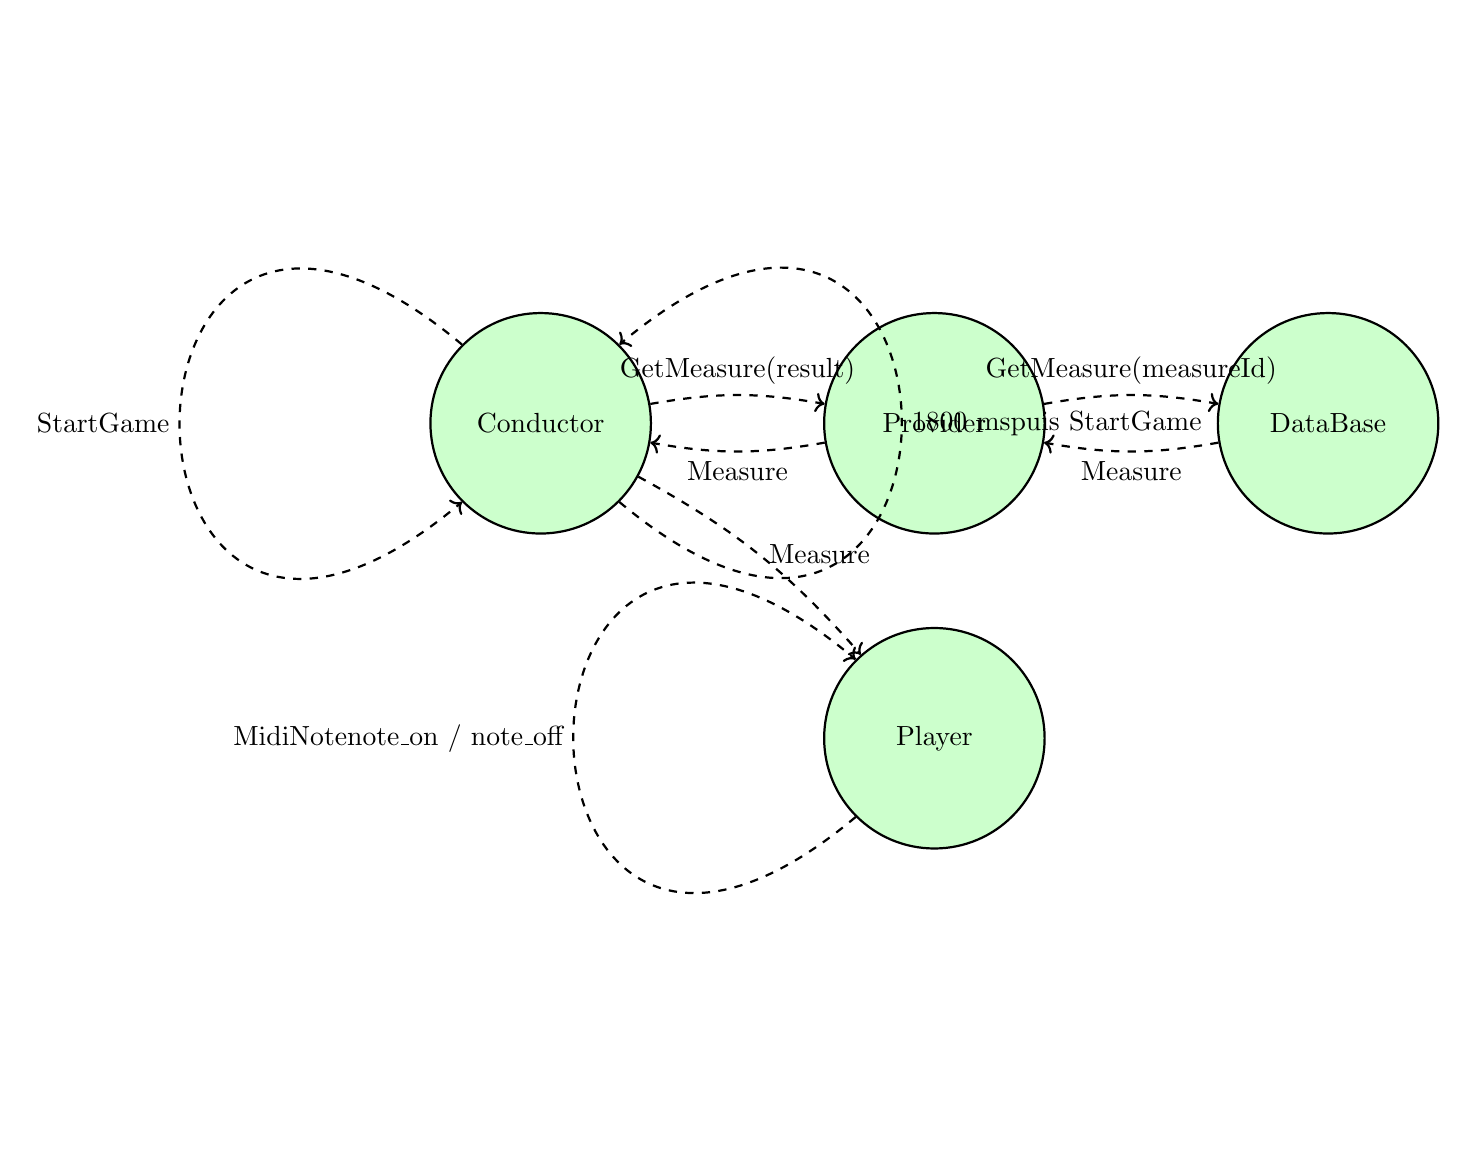
\begin{tikzpicture}[
    actor/.style={
        circle,
        draw,
        thick,
        minimum size=2.8cm,
        align=center,
        fill=green!20
    },
    msg/.style={
        ->,
        dashed,
        thick
    }
]

% Nodes
\node[actor] (conductor) at (0,0) {Conductor};
\node[actor] (provider) at (5,0) {Provider};
\node[actor] (database) at (10,0) {DataBase};
\node[actor] (player) at (5,-4) {Player};

% Messages
\draw[msg] (conductor) to[bend left=10] node[above] {GetMeasure(result)} (provider);
\draw[msg] (provider) to[bend left=10] node[above] {GetMeasure(measureId)} (database);
\draw[msg] (database) to[bend left=10] node[below] {Measure} (provider);
\draw[msg] (provider) to[bend left=10] node[below] {Measure} (conductor);
\draw[msg] (conductor) to[bend left=10] node[right] {Measure} (player);

% Self messages
\draw[msg] (conductor.north west) to[out=140,in=220,looseness=8]
node[left] {StartGame} (conductor.south west);

\draw[msg] (conductor.south east) to[out=320,in=40,looseness=8]
node[right] {1800 ms\\puis StartGame} (conductor.north east);

\draw[msg] (player.south west) to[out=220,in=140,looseness=8]
node[left] {MidiNote\\note\_on / note\_off} (player.north west);

\end{tikzpicture}

\end{document}